\documentclass{article}

\usepackage{graphicx}
\usepackage{graphpap}


\usepackage{fancyhdr}



%%%%%%%%%%%%%%%%%%%%%%%%%%%%%%%%%%%%%%%%5
%
%  Set Up Margins

%%%%%%%%%%%%%%%%%%%%%%%%%%%%%%%%%%%%%%%%%%%%%%%%%
% include file for:
%      Critical Page setup dimensions
%            DO NOT MODIFY
%       (for help see "Latex Line by Line" p 260)
%
\setlength\oddsidemargin{0in}
\setlength\evensidemargin{0in}

\usepackage[left=0.98in, right=0.98in, top=1.0in, bottom=1.0in]{geometry}

% %Top Margin and header
% \setlength\voffset{-0.94in}
% \setlength\topmargin{0.25in}
% \setlength\headheight{0.25in}
% %\setlength\headwidth{6.5in}
% \setlength\headsep{0.25in}
% %Body
% \setlength\textwidth{6.5in}
% \setlength\textheight{9.50in}
% %Footer
% %\setlength\footheight{0.5in}
% \setlength\footskip{0.3750in}
% Line spacing for 6 lines per inch
\linespread{0.894}  % 1.0 = single    1.6 = double
%
%          END of Critical Page Setup Dimensions
%%%%%%%%%%%%%%%%%%%%%%%%%%%%%%%%%%%%%%%%%%%%%%%%%%%

%%%%%%%%%%%%%%%%%%%%%%%%%%%%%%%%%%%%%%%%%%%%%%%%%%%
%
% Useful style and math macros
%


\newcommand\Dfrac[2]{\frac{\displaystyle #1}{\displaystyle #2}}
\newcommand\beq{\begin{equation}}
\newcommand\eeq{\end{equation}}

\newcommand\bmat{\begin{bmatrix}}
\newcommand\emat{\end{bmatrix}}

\newenvironment{solution}
{\vspace{0.125in} {\bf SOLUTION:} \\ }
{\vspace{0.25in}}



%%%%%%%%%%%%%%%%%%%%%%%%%%%%%%%%%%%%%%%%%%%%%%%%%
%
%         Page format Mods HERE
%
%Mod's to page size for this document
\addtolength\textwidth{0cm}
\addtolength\oddsidemargin{0cm}
\addtolength\headsep{0cm}
\addtolength\textheight{0cm}
%\linespread{0.894}   % 0.894 = 6 lines per inch, 1 = "single",  1.6 = "double"

%%%%%%%%%%%%%%%%%%%%%%%%%%%%% HEADER / FOOTER
\pagestyle{fancy}
%%%%%  Page header/footer fields for "NSF Style" proposal
%%%%%  \chead will be changed with each section
\lhead{\small\sc EE543}
\rhead{Wtr 2018}
\chead{HW 2}
\lfoot{Hannaford, U. of Washington}
\rfoot{\today}
\cfoot{\thepage}
%\renewcommand\headrulewidth{1pt}
%\renewcommand\footrulewidth{1pt}

\begin{document}

\setcounter{section}{1}
%%%%** Section 1
\section{Problem Set 2}


Computer software may be used for any problem.   If computer software is used, please state which package you have used and give a concise script in addition to the result.


\subsection{Homogeneous Transforms}
Frames $A$ and $B$ start out superimposed:
\begin{enumerate}
    \item Frame $B$ is translated along $Y_A$ by $L_1$.
    \item Frame $B$ is rotated by $\theta$ around $Z_A$.
    \item Frame $B$ is translated by $L_2$ along $X_B$
    \item Frame $B$ is rotated by $\gamma$ about $Y_B$.
    \item Frame $B$ is translated by $^BV = [v_x,v_y,v_z]^T$
\end{enumerate}

\subsubsection{}
Draw a diagram showing all intermediate frames and their approximate relationships.

\subsubsection{}
Find the resulting 4x4 Homogenous transform $^A_BT$.


\subsection{Homogeneous Transforms}

A car has a roof-attached frame like the car of Example 2.6 (course notes).   The car
\begin{enumerate}
    \item drives in reverse for 10m
    \item turns left by $20^\circ$
    \item drives forward by 20m
    \item turns right by $90^\circ$
    \item goes down a ramp at angle $10^\circ$ for 10m
\end{enumerate}

What is the 4x4 homogenenous transform which represents the position and orientation of the car's frame after these moves?    Assume that all turns can be accomplished without any translation (unlike a real car).



\subsection{Transform Graphs}
An industrial robot must put individual chocolates in a box, $B$, which sits on table, $T$.   The box is located on a table with laser scanner, $S$.

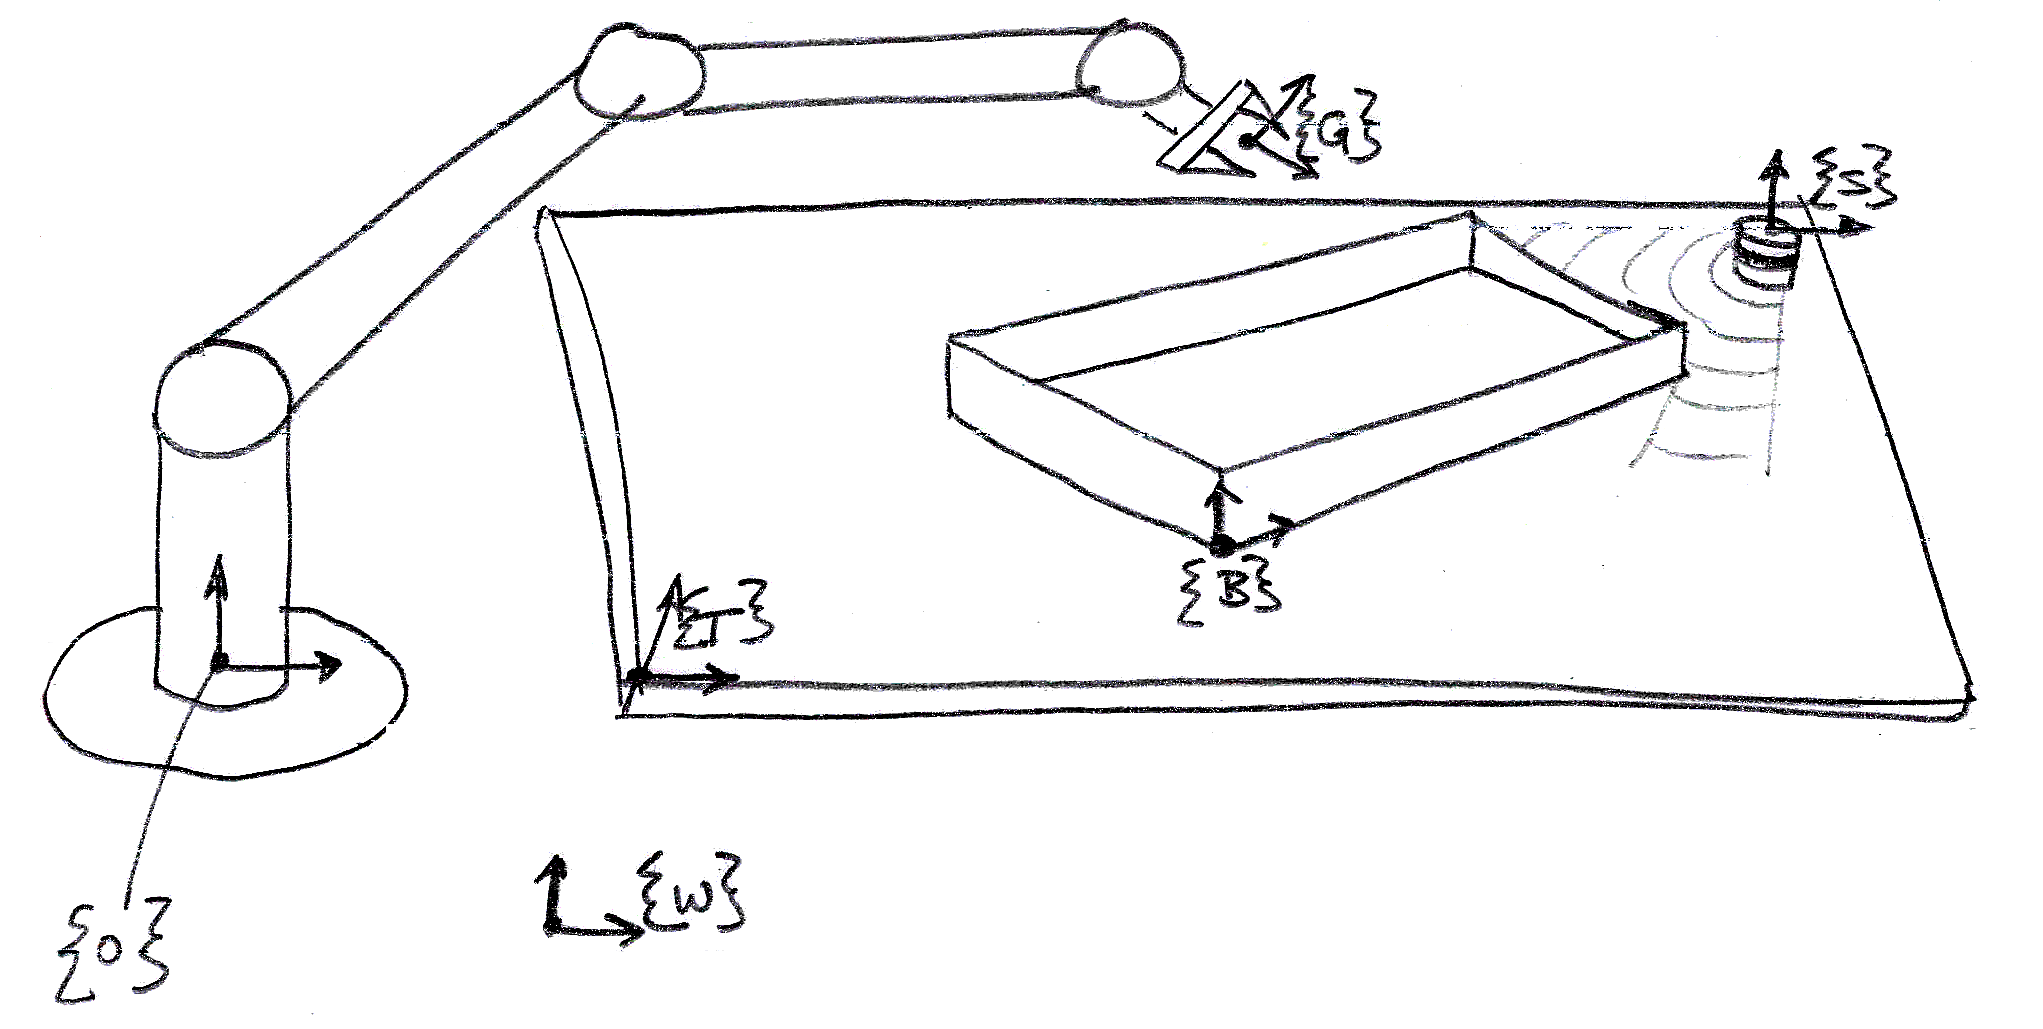
\includegraphics[width=6.5in]{hw1_543_W13_p6a.png}

The following relationships are known:

\[
{^O_GT}\quad{^W_OT}\quad{^T_WT}\quad{^T_ST}\quad{^S_BT}
\]

\subsubsection{}
Draw the transform graph.

\subsubsection{}
Find ${^O_BT}$

\subsubsection{}
Find ${^G_ST}$



%%%%** Section 1.7
\subsection{}

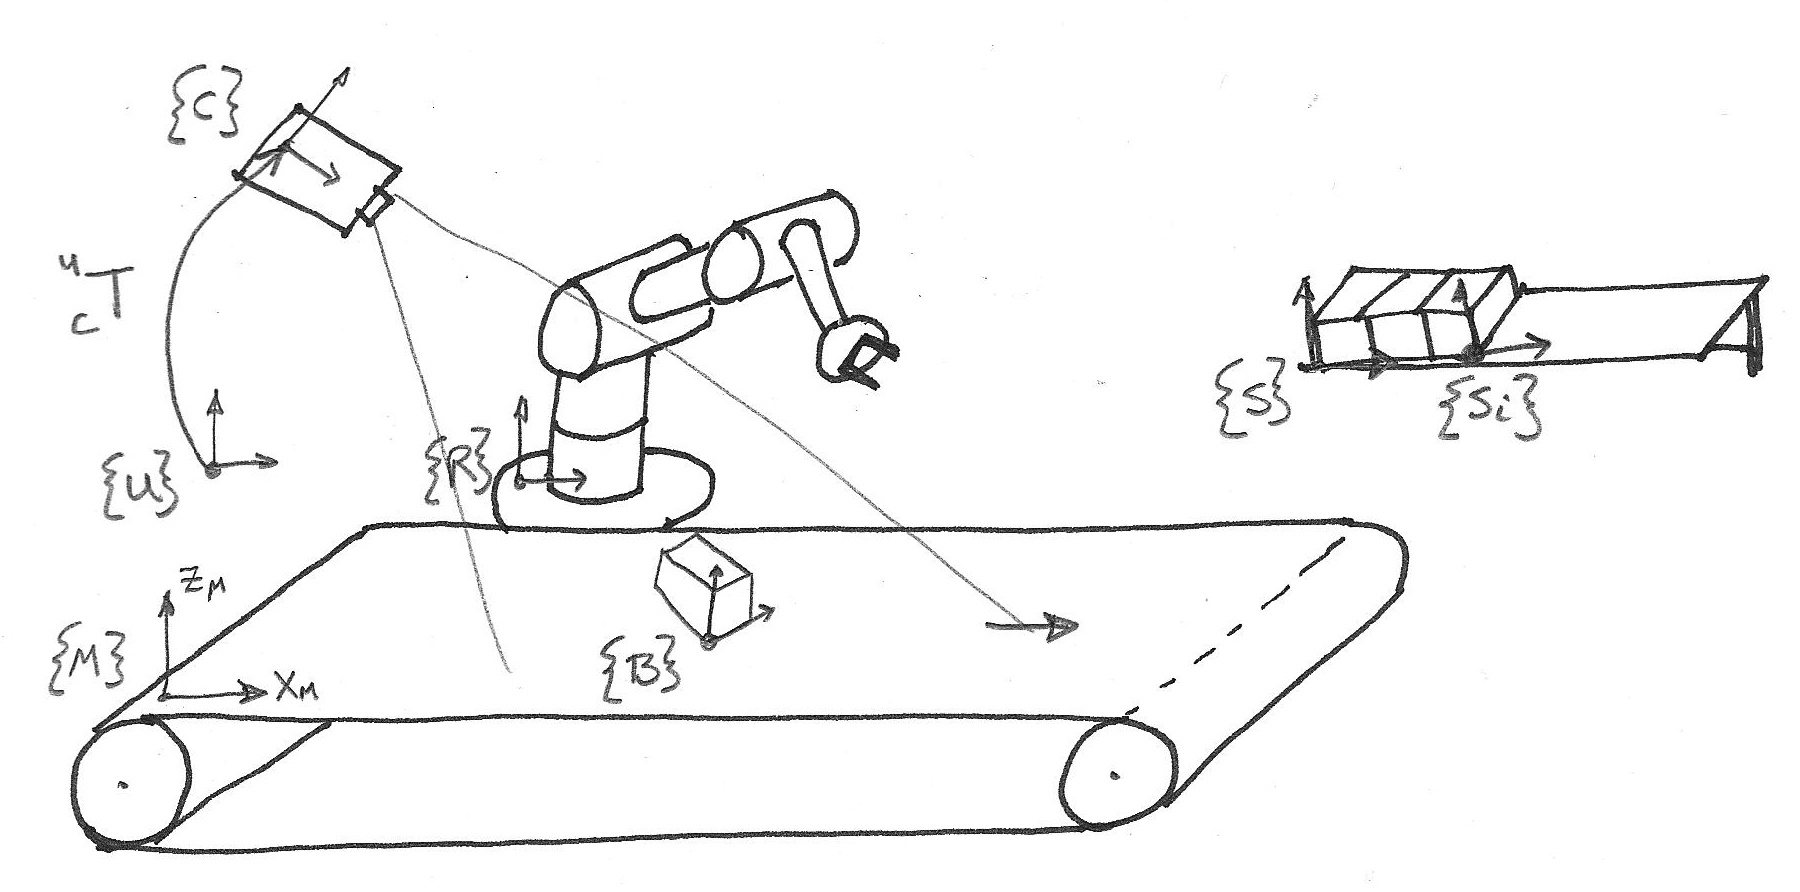
\includegraphics[width=5.0in]{00575.png}

\vspace{0.25in}
A block is on a moving conveyor belt.  We know the following facts and transforms:
\begin{itemize}
  \item ${^U_CT},{^U_ST},{^U_MT},{^U_RT}$
  \item Each block is picked up from the belt and placed on the shelf.  The $i^{th}$ block is stacked to the right (in the $X_S$ direction) starting from frame $S$ when $i=0$.
  \item The block dimensions are $2\times2\times4$ units. They are placed on shelf with two short dimensions facing front.
  \item The camera finds the location of the block, ${^C_BT}$ but after the picture is taken, the belt continues to move in the $X_M$ direction for 0.5 seconds at 0.25 m/sec.
\end{itemize}

\vspace{0.15in}
\subsubsection{}
Find the configuration ${^R_BT}$, of the block in the robot frame after the belt has halted.

\subsubsection{}

Find the configuration of block \#$i$, expressed in frame R.





\end{document}

